\section{Chart::Bars}
\herv{Name:} Chart::Bars\\ \\
\herv{File:} Bars.pm\\ \\
\herv{Requires:}Chart::Base, GD, Carp, FileHandle\\ \\
\herv{Description:} \fett{Bars} is a \fett{subclass} of Chart::Base.\\
The class Bars creates a chart with bars.\\
\\
\herv{Example:}
\begin{figure}[h]
 	\begin{center}
		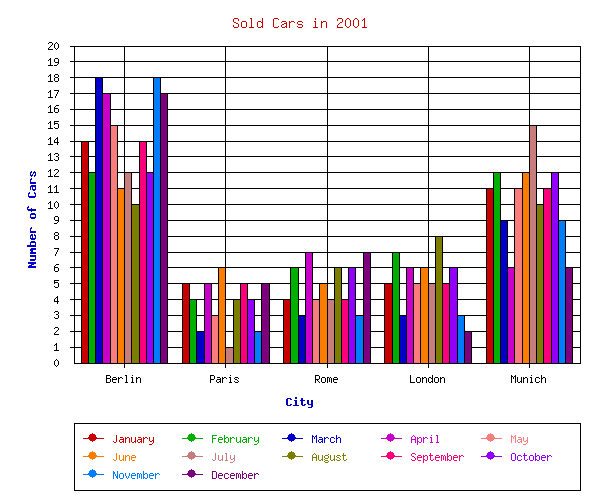
\includegraphics[scale=0.4]{d_bars.png}
	\end{center}
	\caption{Bars chart}
	\label{fig:bars}
\end{figure}
\begin{verbatim}
use Chart::Bars;

$g = Chart::Bars->new(600,500);

$g->add_dataset ('Berlin', 'Paris', 'Rome', 'London', 'Munich');
$g->add_dataset (14, 5, 4, 5, 11);
$g->add_dataset (12, 4, 6, 7, 12);
$g->add_dataset (18, 2, 3, 3, 9);
$g->add_dataset (17, 5, 7, 6, 6);
$g->add_dataset (15, 3, 4, 5, 11);
$g->add_dataset (11, 6, 5, 6, 12);
$g->add_dataset (12, 1, 4, 5, 15);
$g->add_dataset (10, 4, 6, 8, 10);
$g->add_dataset (14, 5, 4, 5, 11);
$g->add_dataset (12, 4, 6, 6, 12);
$g->add_dataset (18, 2, 3, 3, 9);
$g->add_dataset (17, 5, 7, 2, 6);

%hash = ('title' => 'Sold Cars in 2001',
         'text_space' => 5,
         'grey_background' => 'false',
         'integer_ticks_only' => 'true',
         'x_label' => 'City',
         'y_label' => 'Number of Cars',
         'legend' => 'bottom',
         'legend_labels' => ['January' , 'February' , 'March', 'April',
                             'May', 'June', 'July', 'August', 'September',
                             'October', 'November', 'December'],
         'min_val' => 0,
         'max_val' => 20,
         'grid_lines' =>'true',
         'colors' => {'title' => 'red',
                      'x_label' => 'blue',
                      'y_label' => 'blue'} );

$g->set (%hash);

$g->png ("bars.png");

\end{verbatim}
\herv{Constructor:} An instance of a bars chart object can be created with the constructor new():\\
\fett{\$obj = Chart::Bars->new();}\\
\fett{\$obj = Chart::Bars->new(\kursiv{width}, \kursiv{height});}\\
\\
If \fett{new} has no arguments, the constructor returns an image with the size 300x400 pixels. If new has two arguments \kursiv{width} and \kursiv{height}, it returns an image with the desired size. \\ 
\\ 
\herv{Methods:}All universally valid methods, see page \pageref{methods}: Chart::Base. \\
\\
\herv{Attributes/Options:} All universally valid options, see page \pageref{options}. Also available, these special options:
\begin{description}
\item['y\_axes'] Tells chart where to place the y-axis. Valid values are 'left', 'right' and 'both'. Defaults to 'left'.
\item['spaced\_bars']Leaves space between the groups of bars at each data point when set to 'true'.  This just makes it easier to read a bar chart.  Default is 'true'.
\end{description}